\documentclass[]{beamer}
\usepackage[utf8]{inputenc}
\usepackage{hyperref}
\usepackage{listings}
\lstset{
    basicstyle=\fontsize{10}{12}\selectfont\ttfamily,
    keywordstyle=\color{blue},
    breaklines=true,
    showtabs=false,
    showstringspaces=false,
    numberstyle=\tiny\color{mygray}
}
% \usepackage[french]{babel}
% \uselanguage{French}
% \languagepath{French}
\usepackage{pslatex}        % for better PDF on screen
%\usepackage{textcomp}

%\usetheme{AnnArbor}
%\usetheme{Antibes}
%\usetheme{Berkeley}
%\usetheme{Berlin}
%\usetheme{Boadilla}
\usetheme{CambridgeUS}
%\usetheme{Copenhagen}
%\usetheme{Dresden}
%\usetheme{Frankfurt}
%\usetheme{Goettingen}
%\usetheme{Hannover}
%\usetheme{JuanLesPins}
%\usetheme{Marburg}
%\usetheme{Montpellier}
%\usetheme{PaloAlto}
%\usetheme{Pittsburgh}
%\usetheme{Rochester}
%\usetheme{Singapore}
%\usetheme{Szeged}
%\usetheme{Warsaw}



% Set Color ==============================
% Custom colors tested with CambridgeUS.
% If you want a nice looking presentation,
% simply comment this section.
\usepackage{xcolor}

% http://www.computerhope.com/htmcolor.htm
\definecolor{gold}{HTML}{FDD017}
\definecolor{deep sky blue}{HTML}{3BB9FF}
\definecolor{light sky blue}{HTML}{82CAFA}
\definecolor{casesBlue}{HTML}{0072b8}

\makeatletter
\definecolor{mybackground}{HTML}{82CAFA}
\definecolor{myforeground}{HTML}{0000A0}

\setbeamercolor{normal text}{fg=black,bg=white}
\setbeamercolor{alerted text}{fg=red}
\setbeamercolor{example text}{fg=black}

\setbeamercolor{background canvas}{fg=myforeground, bg=white}
\setbeamercolor{background}{fg=myforeground, bg=mybackground}

\setbeamercolor{palette primary}{fg=black, bg=gold}
%       \setbeamercolor{palette secondary}{fg=black, bg=gray!20!white}
\setbeamercolor{palette secondary}{fg=white, bg=casesBlue!80!gold}
\setbeamercolor{palette tertiary}{fg=white, bg=casesBlue}
%       \makeatother

% Set Color ==============================


\hypersetup{
    pdfkeywords = {MONARC, CASES, training, security},
    % pdfpagemode = FullScreen
}

% Navigation menu
% disable options by commenting appropriate line
\setbeamertemplate{navigation symbols}{%
    \insertslidenavigationsymbol
    \insertframenavigationsymbol
    \insertsubsectionnavigationsymbol
    \insertsectionnavigationsymbol
    \insertdocnavigationsymbol
    \insertbackfindforwardnavigationsymbol
}


% contenu de la page de titre
\title[Introduction to MONARC]{Introduction to MONARC}
\subtitle{Optimised Risk Analysis Method}
\author[Team CASES]{Security Made In Lëtzebuerg / CASES}
\institute[]{\href{https://www.cases.lu}{Cyberworld Awareness and Security Enhancements Services}}
\date{February 12, 2020}
% \date{\today{}}
\logo{
\includegraphics[height=0.5cm]{../common_pictures/logo-cases.png}}
\newsavebox{\logoA}
\newsavebox{\logoB}
\savebox{\logoA}{
\includegraphics[width=3.0cm]{../common_pictures/logo-web-cases_lu.png}}
\savebox{\logoB}{
\includegraphics[width=3.0cm]{../common_pictures/logo-monarc-2.png}}
\titlegraphic{%
  \raisebox{.5\dimexpr\ht\logoB-\ht\logoA}{\usebox{\logoA}}% raise smaller logo into position
  \hspace*{5cm}%
  \usebox{\logoB}
}
% End of preamble


\begin{document}
\begin{frame}
    \titlepage
\end{frame}


% Content
%
% SECTION: Luxembourg House of Cybersecurity
%
\section*{Who we are - Our history}
\begin{frame}
%   \frametitle{Luxembourg House of Cybersecurity / Our history}
  \begin{center}
    \begin{itemize}
      \item 2003: Cyberworld Awareness and Security Enhancement Services (\textbf{CASES});
      \item 2007: Computer Incident Response Center Luxembourg (\textbf{CIRCL});
      \item 2010: SECURITYMADEIN.LU is a \textit{GIE} (Groupement d’Intérêt Économique). CIRCL and CASES are department of SECURITYMADEIN.LU;
      \item 2017: Cyber security Competence Center (\textbf{C3}), a new department of SECURITYMADEIN.LU;
      \item On 17th Oct. 2022: SECURITYMADEIN.LU transformed into the Luxembourg House of Cybersecurity (\textbf{LHC}:)\\
        CASES and C3 are now the National Cybersecurity Competence Center of Luxembourg (\textbf{NC3})
    \end{itemize}
  \end{center}
  CASES was an initiative of the Ministry of Economy after the worm
  \textit{I love you} decimated more than 3 millions computers in less than a week.
\end{frame}

% \begin{frame}
%   \frametitle{CASES}
%   \framesubtitle{}
%   \begin{block}{Mission}
%     Foster cyber security by supporting Luxembourg administrations and SMEs.
%   \end{block}
%
%   \begin{block}{Services}
%     \begin{center}
%       \begin{itemize}
%         \item \textbf{Awareness}: publications of articles and videos;
%         \item \textbf{Trainings}:
%         introduction to cyber security for different audiences;
%         \item \textbf{Software}:
%         MONARC, MOSP, Fit4Cybersecurity, etc.
%       \end{itemize}
%     \end{center}
%   \end{block}
%
%   \begin{block}{Cooperations}
%     ANSSI-LU,
%     Centre for Cyber Security Belgium, KonzeptAcht GmbH, ILR, GRC-Luxembourg and others.
%   \end{block}
% \end{frame}

% --------- Summary ---------
\setcounter{tocdepth}{1}
\begin{frame}
  \frametitle{Content at glance}
  \tableofcontents
\end{frame}
\setcounter{tocdepth}{4}
% ----------------------------

%
% SECTION: What is MONARC?
%
\section{What is MONARC?}
\begin{frame}
  \frametitle{Summary}
  \tableofcontents[currentsection, hideothersubsections]
\end{frame}
\subsection{An open source software}
\begin{frame}
  \frametitle{An open source software}
  \framesubtitle{}
  MONARC is the tool you need for an optimised, precise and repeatable risk assessment.

  \bigskip
  \begin{itemize}
    \item Web application (SaaS, self-hosted, virtual machine, etc.);
    \item source code\footnote{\url{https://github.com/monarc-project}}:
    \texttt{GNU Affero General Public License version 3};
    \item data: \texttt{CC0 1.0 Universal - Public Domain Dedication}.
  \end{itemize}

  \bigskip
  MONARC is easy to use.

  Used and recognized by experts from different fields (not only information security).

  \bigskip
  For many users, it started with a spreadsheet!
\end{frame}

\subsection{A community}
\begin{frame}
  \frametitle{A community}
  \framesubtitle{}
  \begin{itemize}
    \item more than 260 organizations:\\ \url{https://my.monarc.lu};
    \item 17 organizations sharing MONARC objects (threats, assets, recommendations, etc.):\\
    \url{https://objects.monarc.lu};
    \item a global dashboard with trends about threats and vulnerabilitties:\\
    \url{https://dashboard.monarc.lu};
    \item discussions on GitHub:\\
    \url{https://github.com/monarc-project/MonarcAppFO/discussions}.
  \end{itemize}
\end{frame}

\subsection{A method}
\begin{frame}
  \frametitle{A method}
  \framesubtitle{Based on \texttt{ISO/IEC 27005:2011}, but optimized}
  \begin{center}
    \includegraphics[scale=0.6]{../common_pictures/iso27005-2011.png}
  \end{center}
\end{frame}


%
% SECTION: The method
%
\section{The method}
\begin{frame}
    \frametitle{Summary}
    \tableofcontents[currentsection, hideothersubsections]
\end{frame}


\subsection{Management of risk}
\begin{frame}
    \frametitle{A Structured, Iterative and Qualitative method}
    \framesubtitle{}
    \begin{columns}[t]
        \column{5.5cm}
        \begin{figure}
        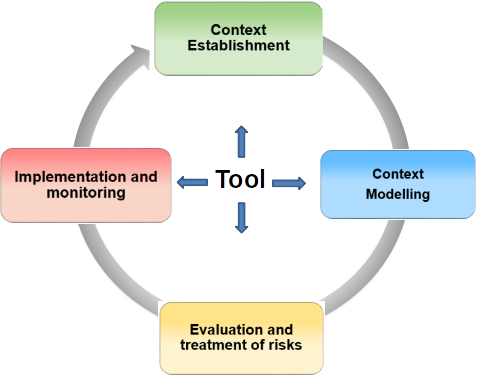
\includegraphics[width=5.5cm]{./images/MONARC-method-1.png}
        \end{figure}
        \column{6.5cm}
        \begin{itemize}
                \item Structured: 1, 2, ..., n.
                \item Iterative: \textbf{Plan}, \textbf{Do}, \textbf{Check}, \textbf{Act}
                \item Qualitative: \textbf{Values} / \textbf{Consequence}
                    \begin{itemize}
                        \item Impact/Consequence, Threat, Vulnerability;
                        \item \textbf{r}eputation, image;
                        \item \textbf{o}peration;
                        \item \textbf{l}egal;
                        \item \textbf{f}inancial;
                        \item \textbf{p}erson (to the).
                    \end{itemize}
        \end{itemize}
        \end{columns}

\end{frame}

\begin{frame}
    \frametitle{Automated and simplified management}
    \framesubtitle{Method based on \texttt{ISO/IEC 27005}}
    \begin{center}
        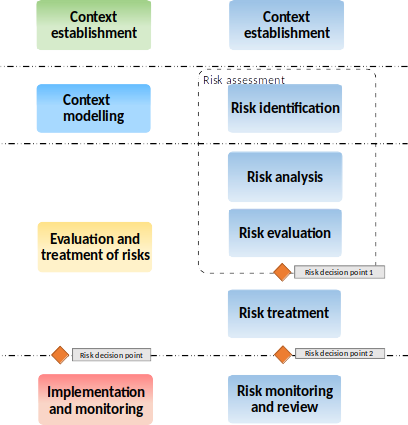
\includegraphics[scale=0.45]{./images/MONARC-method-2-2.png}
    \end{center}
\end{frame}

\begin{frame}
    \frametitle{Automated and simplified management}
    \framesubtitle{Sub-stages provided by the method are also in line with \texttt{ISO/IEC 27005}}
    \begin{center}
        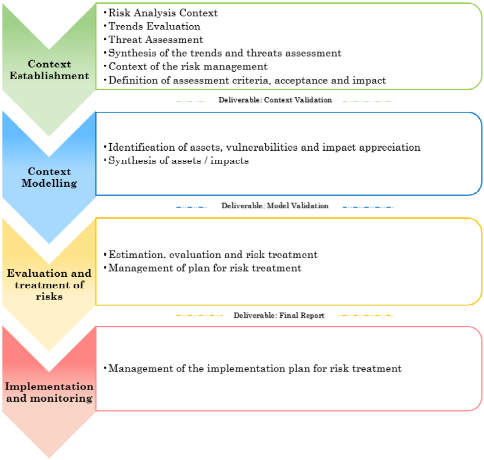
\includegraphics[scale=0.4]{./images/MONARC-method-2-1.png}
    \end{center}
\end{frame}

\begin{frame}
    \frametitle{ISO/IEC 27005:2011}
    \framesubtitle{Information risks}
    \begin{block}{Formula}
        $$R = I \times T \times V$$
        \begin{itemize}
            \item impact on \textbf{C}onfidentiality \textbf{I}ntegrity \textbf{A}vailability;
            \item on secondary assets.
        \end{itemize}
    \end{block}
\end{frame}


\begin{frame}
    \frametitle{ISO/IEC 27005:2011}
    \framesubtitle{Operational risks}
    \begin{block}{Formula}
        $$R = I \times P$$
        \begin{itemize}
            \item impact on ROLFP;
            \item on primary assets.
        \end{itemize}
    \end{block}
\end{frame}


\subsection{An optimized method}
\begin{frame}
    \frametitle{Optimizations}
    \framesubtitle{}
    MONARC is an optimized method:
    \begin{itemize}
        \item inheritance;
        \item scope of objects;
        \item models;
        \item deliverables.
    \end{itemize}
\end{frame}

\subsubsection{Inheritance}
\begin{frame}
    \frametitle{Inheritance}
    \framesubtitle{Modelling}
    \begin{center}
        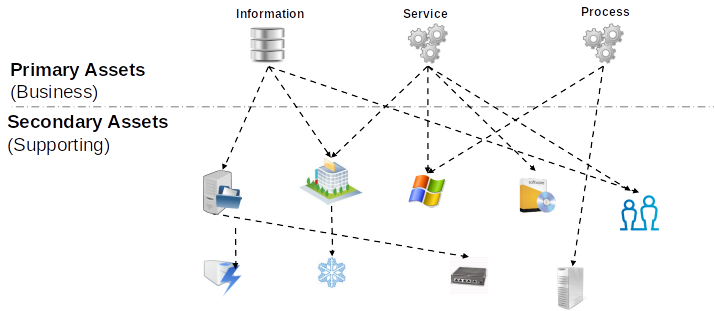
\includegraphics[scale=0.45]{./images/MONARC-method-modelling.png}
    \end{center}
\end{frame}

\begin{frame}
    \frametitle{Inheritance}
    \framesubtitle{Formalisation of the modelling}
    \begin{center}
        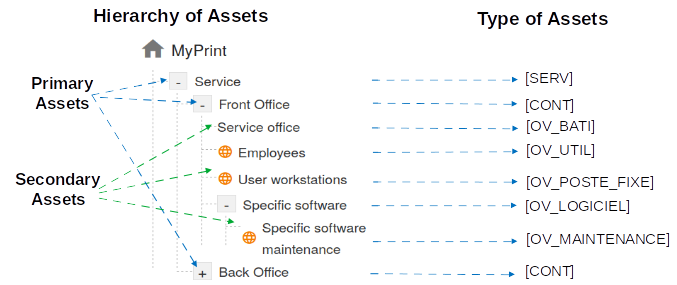
\includegraphics[scale=0.5]{./images/MONARC-modelling-formalisation.png}
    \end{center}
\end{frame}

\begin{frame}
    \frametitle{Inheritance}
    \framesubtitle{Formalisation of an asset}
    Example with \texttt{OV\_BATI}
    \begin{center}
        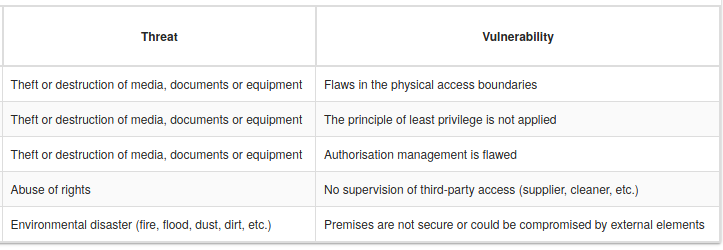
\includegraphics[scale=0.7]{./images/ov_bati.png}
    \end{center}
\end{frame}

\subsubsection{Scope of objects}
\begin{frame}
    \frametitle{Scope of objects}
    \framesubtitle{Global or local assets}
    \begin{center}
        \begin{center}
            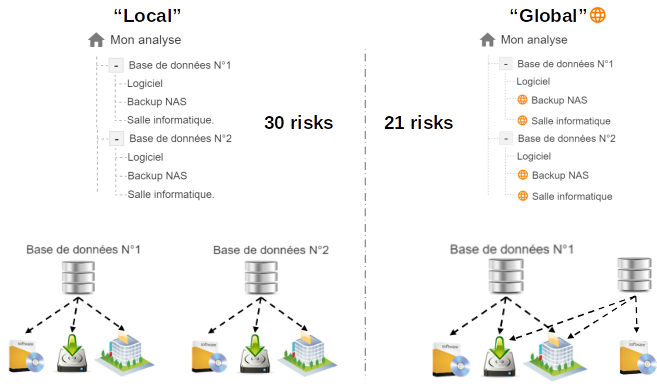
\includegraphics[scale=0.45]{./images/global-vs-local.png}
        \end{center}
    \end{center}
\end{frame}

\subsubsection{Inheritance}
\begin{frame}
    \frametitle{Inheritance of impacts}
    \framesubtitle{}
    \begin{center}
        \begin{center}
            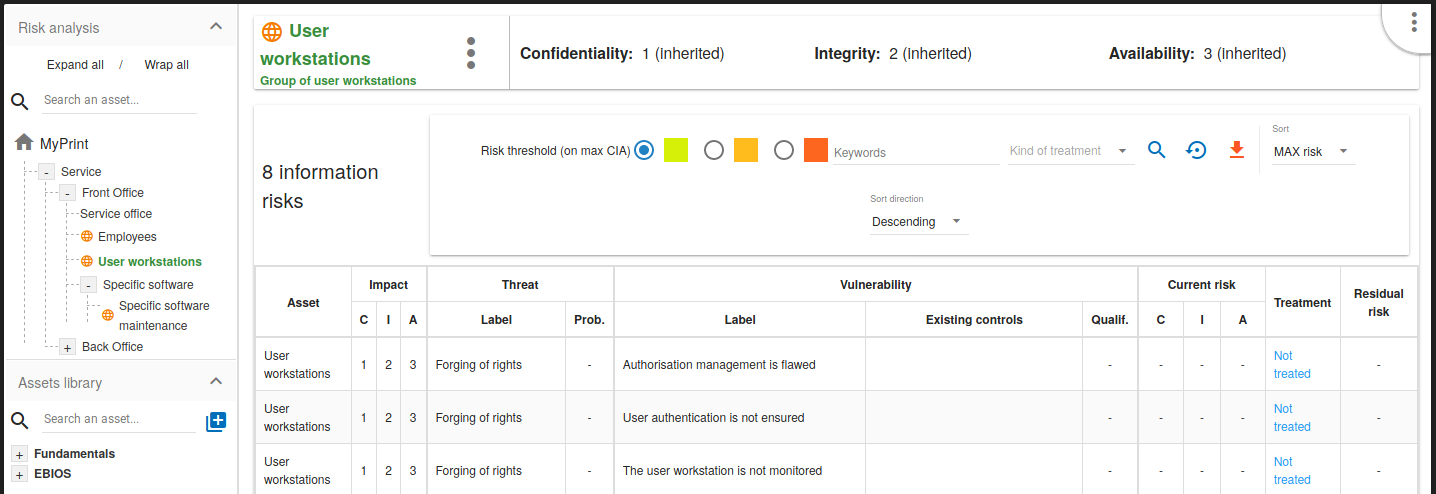
\includegraphics[width=12cm]{./images/impacts-inheritance.png}
        \end{center}
    \end{center}
\end{frame}

\subsubsection{Deliverables}
\begin{frame}
    \frametitle{Deliverables}
    \framesubtitle{}
    Shareable templates of deliverables.
\end{frame}

%
% SECTION: The tool
%
\section{The tool}
\begin{frame}
    \frametitle{Summary}
    \tableofcontents[currentsection, hideothersubsections]
\end{frame}
\subsection{Architecture}
\begin{frame}
    \frametitle{}
    \framesubtitle{}
    \begin{center}
        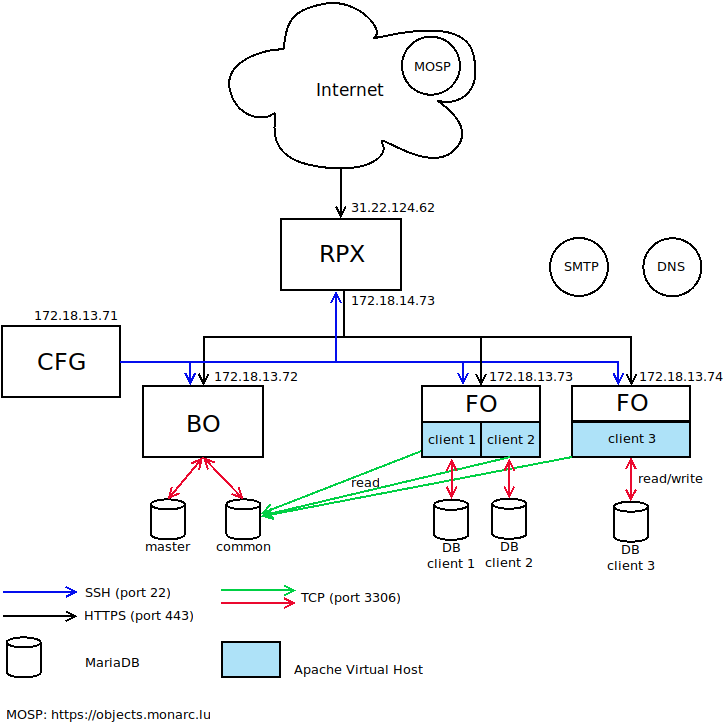
\includegraphics[scale=0.3]{../common_pictures/monarc-architecture.png}
    \end{center}
\end{frame}



\subsection{Workshop}
\begin{frame}
    \frametitle{Le'ts work a little!}
    \framesubtitle{}
    \begin{itemize}
      \item training instance: \url{https://formation.monarc.lu}
      \item login: \texttt{user\_X@monarc.lu}, where $01 \leq X \leq 30$;
      \item password: \texttt{Password1234!}
    \end{itemize}

    \bigskip
    Preferably use Firefox, alternatively Chrome. But not Internet Explorer.
\end{frame}



\subsection{Modules}
\subsubsection{Dashboard}
\begin{frame}
    \frametitle{Dashboard}
    \framesubtitle{}
    \begin{itemize}
        \item provide different visualizations of the current analysis state;
        \item visualizations are exportable (.png, .csv, .pptx).
    \end{itemize}
\end{frame}

\subsubsection{Statement of Applicabitity}
\begin{frame}
    \frametitle{Statement of Applicabitity}
    \framesubtitle{}
    Statement of Applicability (SOA) and compliance level for a referential security.
\end{frame}

\subsubsection{Record of processing activities}
\begin{frame}
    \frametitle{Record of processing activities}
    \framesubtitle{}
    Register of the information treatment for processing activities.
\end{frame}



\subsection{Roadmap}
\subsubsection{Past}
\begin{frame}
    \frametitle{Latest notable developments}
    \framesubtitle{}
    \begin{itemize}
      \item statement of applicability (\href{https://www.monarc.lu/news/2018/08/22/monarc-270-released/}{MONARC 2.7.0});
      \item connection with MOSP (\href{https://www.monarc.lu/news/2019/05/28/monarc-282-released/}{MONARC 2.8.2});
      \item records of processing activities for the GDPR (\href{https://www.monarc.lu/news/2019/08/23/monarc-290-released/}{MONARC 2.9.0});
      \item management of set of recommendations (\href{https://www.monarc.lu/news/2019/08/23/monarc-290-released/}{MONARC 2.9.0});
      \item port of the backend to Zend Framework 3 (\href{https://www.monarc.lu/news/2019/11/25/monarc-291-released/}{MONARC 2.9.1});  
      \item new dashboard for the CEO role: global dashboard with data gathered from different MONARC instances. (MONARC 2.10.1);
      \item definition of custom scales for operational risks (\href{https://www.monarc.lu/news/2021/09/02/monarc-2110-released/}{2.11.0}).
    \end{itemize}
\end{frame}

\subsubsection{Future}
\begin{frame}
    \frametitle{Future developments}
    \framesubtitle{}
    \begin{itemize}
        \item improvements of the new global dashboard towards a security weather forecast (ongoing development);
        \item enhancements to the sharing of MONARC objects with MOSP\footnote{\url{https://objects.monarc.lu}} (ongoing development);
        \item link between GDPR module and some objects in MONARC;
        \item new front-end.
    \end{itemize}
    \bigskip
    Idea ?
    $\rightarrow$
    \href{https://github.com/monarc-project/MonarcAppFO/issues/new?labels=feature+request}{Feature request}
\end{frame}

% %
% SECTION: Modules
%
\section{Modules}
\begin{frame}
    \frametitle{Summary}
    \begin{columns}[t]
        \begin{column}{5cm}
            \tableofcontents[sections={1-3}, currentsection, hideothersubsections]
        \end{column}
        \begin{column}{5cm}
            \tableofcontents[sections={4-5}, currentsection, hideothersubsections]
        \end{column}
    \end{columns}
\end{frame}
\subsection{Dashboard}
\begin{frame}
    \frametitle{}
    \framesubtitle{}
\end{frame}


\subsection{Statement of Applicabitity}
\begin{frame}
    \frametitle{}
    \framesubtitle{}
\end{frame}


\subsection{Record of processing activities}
\begin{frame}
    \frametitle{}
    \framesubtitle{}
\end{frame}

% %
% SECTION: Roadmap
%
\section{Roadmap}
\begin{frame}
    \frametitle{Summary}
    \begin{columns}[t]
        \begin{column}{5cm}
            \tableofcontents[sections={1-3}, currentsection, hideothersubsections]
        \end{column}
        \begin{column}{5cm}
            \tableofcontents[sections={4-6}, currentsection, hideothersubsections]
        \end{column}
    \end{columns}
\end{frame}

\subsection{Past}
\begin{frame}
    \frametitle{Latest notable developments}
    \framesubtitle{}
    \begin{itemize}
        \item records of processing activities for the GDPR (MONARC 2.9.0);
        \item management of set of recommendations (MONARC 2.9.0);
        \item connection with MOSP (MONARC 2.8.2);
        \item statement of applicability (MONARC 2.7.0).
    \end{itemize}
    \bigskip
    Current version of MONARC is 2.9.9.
\end{frame}

\subsection{Future}
\begin{frame}
    \frametitle{Future developments}
    \framesubtitle{}
    \begin{itemize}
        \item LDAP;
        \item Single Sign On;
        \item new front-end;
    \end{itemize}
\end{frame}

%
% SECTION: Services
%
\section*{Services}
\begin{frame}
    \frametitle{Services related to MONARC}
    \begin{center}
        \begin{itemize}
            \item help at deploying;
            \item help at using;
            \item trainings;
            \item developments, feature requests.
        \end{itemize}
    \end{center}
\end{frame} 



%
% SECTION: End of the presentation
%
\section*{End of the presentation}
\begin{frame}
    \frametitle{End of the presentation}
    \framesubtitle{}
    \begin{center}
        \begin{itemize}
            \item Thank you for listening.
            \item Contact: info@cases.lu
            \item \url{https://github.com/monarc-project}
            \item \url{https://www.monarc.lu}
        \end{itemize}
    \end{center}
\end{frame}
\end{document}
